\section{Overview}
\label{overview}

\subsection{Conceptual introduction}
\label{conceptual introduction}

\subsubsection{Motivation and applications}

I will take as a definition \textit{topological quantum information} to be the study of information in topological quantum systems. A topological quantum system is some mathematical or physical system which is in a fundamental sense described by the mathematics of both quantum mechanics and topology. The term \textit{quantum system} here is used in contrast to \textit{classical system}. The flow of current through a conducting copper wire is described perfectly well by classical electromagnetism, whereas the flow of current through a superconducting niobium-titanium wire necessarily requires quantum mechanics for its description.

The term \textit{topological system} is used in contrast to \textit{geometric systems}, though the term “geometric system” is a nonstandard one. In a geometric system measurable quantities and phenomena depend on quantitative local aspects of the system - the distance between wires, the exact shape of some sample, or the curvature of some component. In a topological system measurable quantities and phenomena depend only on qualitative global aspects of the system - whether two wires cross or not, whether a sample is connected or not, whether a component curves into a ball or has a boundary.

I say that this book is about “topological quantum information” and not “topological quantum systems” for two reasons. The first is to highlight the fact that there is more to a topological quantum systems than its global topological properties. Topological quantum systems also have local geometric descriptions which are important for understanding many phenomina. However, we will mostly be ignoring these local effects in favor of focusing on global topological properties. The beauty of topological quantum systems lies exactly in the fact that this global perspective retains all the essential information in the system. The second reason is to highlight this book’s eye towards topological quantum computing, the idea of making computers using topological quantum systems. 

Since Peter Shor’s 1994 discovery of an efficient factoring algorithm on quantum computers \cite{shor1994algorithms}, the primary goal of quantum information theorists has been to harness quantum information sufficiently well so that it can be used to make an efficient scalable quantum computer. One of the major hurdles in achieving this goal is that quantum information is \textit{fragile}. Small amounts of noise coming from nearby electromagnetic fields or imperfections in experimental devices are often enough to affect the information being stored, resulting in \textit{errors} in the computation. In the early days of quantum computing it was not clear whether there was any way around this problem. Perhaps the inherent fragility of quantum information would make quantum computation impossible. This turned out to be false.

The beautiful observation is that errors are not nearly as catastrophic in \textit{topological} quantum systems. Errors are typically local. By definition the information topological systems does not depend on local properties, and hence is not affected by local changes. Hence, under suitable conditions, topological systems are naturally error resistant! In the same way that invariants of topological spaces are supposed to be invariant under deformations in pure mathematics, information in topological systems is invariant under errors in mathematical physics. Hence, to solve the problem of noise all one has to do is make a \textit{topological} quantum computer! This observation was made in 1997 and is due independently to Alexei Kitaev and Michael Freedman \cite{kitaev2003fault, freedman1998p}. Since then topological quantum computing has grown and evolved, finding its way into almost every modern proposal for fault-tolerant quantum computing.

The first approach to topological quantum computing is to use a physical material, some literal condensed collection of atoms, which naturally behaves as a topological quantum system. These exist and have been studied for a long time. For instance, a two dimensional sheet of graphene behaves topologically when it is subjected to low temperatures ($\approx$5 degrees Kelvin) and large magnetic fields ($\approx$15 Teslas) \cite{bolotin2009observation}. Topological quantum materials which can be used to make scalable quantum computers require intricate experiments to operate, which has been the most prominent roadblock in this approach.

The second approach to topological quantum computing is to artificially construct a topological system within a geometric one. The function of a quantum computer, almost by definition, is to simulate quantum systems. In particular, it can simulate \textit{topological} quantum systems. Since topological systems are resistant to local errors, this means that the original computer which is simulating the topological system will itself become resistant to local noise! This works exactly as described as long as the simulation itself is local, that is, local effects in the original system correspond to local effects in the simulated system. This technique of simulating topological systems to inherit their error-resistant properties is known as \textit{topological quantum error correction}. The advantage of this approach is that it works on any hardware available. The disadvantage is that to perform useful computations one must pass through simulation involved the topological quantum error correction. This additional layer adds a hefty amount of overhead, which can eat up the majority of runtime and resources. It is for this reason that \textit{efficient} topological quantum error correction is an important and active area of research.

\begin{figure}
\[\begin{tikzcd}
	& \begin{array}{c} \substack{\text{topological}\\ \text{quantum}\\\text{materials}} \end{array} \\
	\begin{array}{c} \substack{\text{topological} \\ \text{quantum} \\ \text{information}} \end{array} \\
	& \begin{array}{c} \substack{\text{topological}\\\text{quantum}\\ \text{error correction}} \end{array}
	\arrow["\begin{array}{c} \substack{\text{intrinsic}\\\text{realization}} \end{array}", from=2-1, to=1-2]
	\arrow["\begin{array}{c} \substack{\text{local}\\\text{simulation}} \end{array}"', from=2-1, to=3-2]
\end{tikzcd}\]
\caption{The two major branches of topological quantum information.}
\end{figure}

Of course, the above discussion presents only one motivation for topological quantum information and only one example of an application. Topological quantum materials open a whole world of potential applications, and it seems they may play an important role in the techonologies of the future \cite{ramirez2020dawn}. Some proposed applications include processing classical information using topological defects in magnetic devices (with the end goal of making high-speed low-energy transmissions) \cite{marrows2021perspective, vsmejkal2018topological}, creating highly sensitive photodetectors (with the end goal of making night-vision goggles or sensors) \cite{chan2017photocurrents}, creating technolgies with high thermoelectric effect (with the end goal of making efficient fridges or electric generators) \cite{skinner2018large}, creating highly-efficient transistors \cite{fuhrer2021proposal}, and engineering tiny electrical components \cite{viola2014hall, placke2017model}. 

This breadth of potential applications is due in part to the number of different types of topological materials which have been discovered or theorized. This includes quantized Hall states \cite{von202040}, topological insulators \cite{hasan2010colloquium}, fractional Chern insulators \cite{regnault2011fractional}, Weyl/Dirac semimetals \cite{armitage2018weyl}, and topological superconductors \cite{sato2017topological}. The contents of this book certainly do not provide the entire picture for any of these materials. However, the hope is that it gives a picture of the algebraic structures within them, hence helping readers think both concretely and conceptually about these materials and their applications.

\subsubsection{Mathematical picture}

The term \textit{topological quantum system} is broad. To get a rigorous mathematical subject, we will focus on a specific type of topological quantum system known as a \textit{topologically ordered} quantum system. Topological order is much more precise, though there are still conflicting definitions in the literature. Specifically, I will be focusing on \textit{(2+1)-dimensional} topological order. Here, I am using the physicist convention of using (2+1)D to refer to two space dimensions and one time dimension. That is, I will be discussing a locally flat topologically ordered system. For example, a single sheet of graphene at low temperatures and large magnetic fields can exhibit a form of (2+1)D topological order, and any quantum computer running topological quantum error correction can also exhibits a form of (2+1)D topological order.

\begin{center}
\fbox{All systems in this book are two-dimensional unless stated otherwise.}
\end{center}

Topological quantum systems can be described in many different ways. In this book we will take an \textit{algebraic} approach. [WORK: what does it mean to take an algebraic approach to something?]. The algebraic structure which houses the algebraic data of a (2+1)D topologically ordered system is known as a \textit{modular tensor category}. These algebraic structures are the main mathematical object of this text. Once one has a modular tensor category it is easy to manipulate the stored information to perform computations. This gives us the overall schema of our mathematical discussion, illustrated visually below:

\begin{equation*}
\tikzfig{mathematical-outline}
\end{equation*}

In Chapter [ref] we describe topological order. In Chapter [ref] we describe topological order algebraically in terms of modular tensor categories. In Chapter [ref] we describe further algebraic structures which lie beyond plain modular tensor categories, which allow us to describe more complex behaviors in topological order. Finally, in Chapter [ref] we will use the tools we have established to detail several algorithms and procedures for topological quantum computaiton. Two introductory chapters are also included: Chapter [ref] which establishes the theory of finite dimensional quantum systems and Chapter [ref] which establishes category theory.

\subsubsection{History of the subject}

Like with any sufficiently rich subject, the history of topological quantum information can be traced back as far as one wants. So let us do exactly that. The first use of topology in information science was roughly 2600 BCE, with the South American \textit{Quipu} \cite{ascher1981code}. Quipu are intricate knotted strings typically made out of cotton fibers. The knots in the string are used to store various types of information, typically numbers. Mathematically we say that Quipu store their information in knot invariants, and hence hold \textit{topological} information.

Quipu were so successful that they remained the primary method of information processing in much of South America for thousands of years. They reached their peak of usage in the 15th century via the Inca empire. The Inca empire was the largest pre-Columbian empire in the western hemisphere, with over ten million subjects and spanning over two million square kilometers. Despite their intricate government, the Incas had \textit{no written language}. This distinguished them from their contemporary empires, such as the Mali, Mongolian, or Chinese empires, which all relied on the written word. The success of the Inca empire can be seen as a testament to the versatility and power of knot invariants. The difference between the Inca and modern proposals for topological quantum computers is that instead of the strings being made out of cotton fibers they are made out of the spacetime trajectories of quasiparticles in topological systems.

Just like the history of topology in information science can be traced back to the origin of information science, the history of topology in quantum mechanics can be traced back to the origins of quantum mechanics. There is a 1931 paper of Paul Dirac \cite{dirac1931quantised} which introduces many of the ideas which would become foundational to topological quantum mechanics. In the 1950s, explicitly topological ideas such as the Aharanov-Bohm effect \cite{aharonov1959significance} and the theory of point defects by Tony Skyrme \cite{skyrme1962unified} were beginning to emerge. By the 1970s nontrivial abstract topological considerations were leading to novel contributions to contemporary physics, such as the theoretical description of the A-phase of superfluid Helium-3 \cite{anderson1977phase} and the theory of phase transitions in the xy model proposed by Kosterlitz-Thouless \cite{kosterlitz1973ordering}. These results were associated with the 1996 and 2016 Nobel prize respectively.

It was in the 1980s, however, that topology established itself as one of the leading themes in condensed matter physics. The discovery of the quantum Hall effect in 1980 \cite{klitzing1980new} and the subsequent discovery of the fractional quantum Hall effect in 1982 \cite{tsui1982two} gave the first examples of topologically ordered systems in our modern sense of the word, and resulted in the 1985 and 1998 Nobel prizes respectively. These systems gave theorists the license to dream big about what possibilities could lie ahead. This led to major work by theorists such as Frank Wilczek \cite{wilczek1982quantum, arovas1985statistical}, Duncan Haldane \cite{haldane1983nonlinear, haldane1988model}, and others on the theory of topological quantum systems.

The most notable of these theorists for our present story is Edward Witten, with his introduction of \textit{topological quantum field theory} in 1988 \cite{witten1988topological}. This work not only put the modern experiments within a larger context, but it also connected these developments to a parallel story which had been developing within pure mathematics. Namely, knot theory. In 1984 Vaughn Jones discovered his landmark knot invariant, which was powerful in its ability to distinguish between non-equivalent knots \cite{jones1997polynomial}. This marked the first major progress in the field since Alexander's invariant in 1928 \cite{alexander1928topological}. However, Jones’ construction was steeped in opaque subfactor theory, so much so that the fact that it resulted in knot invariant felt almost like a happy accident. Hence, a widespread topic on the mind of contemporary mathematicians was how to properly interpret the Jones invariant, and how to construct other invariants like it. Witten seemed to answer both. After defining topological quantum field theory, he showed how the Jones invariant could be obtained as an observable quantity within a certain field theory \cite{witten1989quantum}! This shocking result gave a new interpretation of the Jones invariant in terms of mathematical physics which was appealing to experts. Seeing as the Jones invariant was constructed from a topological quantum field theory, it was natural to expect that other field theories might give new invariants which could distinguish between even more knots. This vision of invariants in low-dimensional topology constructed using topological quantum field theory became known as \textit{quantum topology}, and evolved into its own discipline in the following years.

This brings us to 1997. Quantum topology is an active area in pure mathematics, and topological themes in condensed matter physics are at the forefront of the field. The open problem is how to construct a fault tolerant quantum computer. Peter Shor had recently discovered his factoring algorithm \cite{shor1994algorithms}, and there was debate about whether scalable quantum error correction was possible \cite{landauer1995quantum}. This led to two independent proposals for topological quantum computation in the same year. One was by the mathematician Michael Freedman \cite{freedman1998p}. His vision was clear. A recent paper had shown that computing the Jones invariant of knots was in general an NP-hard problem \cite{jaeger1990computational}. However, by the work of Witten, the Jones invariants of knots were observables in certain topological quantum field theories. Hence, if one could construct physically a topologically ordered system which was described by Witten’s topological quantum field theory then the Jones polynomial of knots could be computed efficiently by making measurements on the system. Hence, one would obtain a very powerful computer! This was Freedman’s proposal.

The other proposal was made by theoretical physicist Alexei Kitaev \cite{kitaev2003fault}. His proposal was much more precise. He gave a toy model for a certain family of topologically ordered systems. He then outlined a technique for storing and manipulating information within these systems. The deep observation was that these systems were intricate enough that they could be used to make a powerful quantum computer \cite{mochon2003anyons}.

In the subsequent years Freedman and Kitaev teamed up with collaborators Zhenghan Wang, Michael Larsen, and others to study the new field of topological quantum information and the possibility of constructing a topological quantum computer. One of the first major results was that no topological quantum computer could be more powerful than a standard quantum computer \cite{freedman2002simulation}. This went against Freedman’s original hope to solve NP-hard problems using topological quantum computers. Freedman’s mistake was in asserting that topological quantum computers could compute the Jones polynomial. The measurements which give the Jones invariant in topological quantum field theory will always be \textit{approximate}. Approximating the Jones invariant in this way is computationally easier than evaluating the Jones invariant exactly. In fact, this way of approximating the Jones invariant is \textit{not} NP-hard - it can only be used to solve problems which could efficiently be solved using standard quantum computers.

The second major result of Freedman, Kitaev, Wang, and Larsen was the converse of their first result \cite{freedman2002modular}. Namely, they showed that every quantum algorithm can be efficiently run on a topological quantum computer. They do this by showing that every quantum algorithm can be efficiently reinterpreted in terms of computing the Jones invariant of some knot. In this way computing the Jones invariant is not NP-hard, but it is a \textit{universal problem} for quantum computation. They then formalize Freedman’s ideas about topological quantum field theory, and show directly that realistic operations on a topologically ordered quantum system described by Witten’s quantum field theory can be used to compute the Jones invariants of knots.

Together, these two results show in a real sense that topological quantum computing is equally powerful as standard quantum computing with quantum circuits. This laid the groundwork for fruitful studies of fault-tolerant topological quantum computing, both using error correcting codes and physical materials. This has resulted in a great number of important results, which we will discuss at length throughout the rest of this manuscript.

\subsection{Technical introduction}
\label{technical introduction}

\subsubsection{Principles of topological quantum information}

In this section we will lay out the general principles of topological quantum information. As an organizational tool, these principles are introduced one by one as we construct a sample topological system. This example is meant to be representative of the systems we will encounter throughout this text, and within the broader field of topological quantum information. As a further organization tool, this example is constructed with the stated goal of obtaining a topological quantum computer.

Our system will be flat, containing only two spatial dimensions. Our system will be mostly homogenous, essentially identical everywhere, at the exception of finitely many localized regions. These regions will differ substantially from the top-dimensional homogeneous bulk. These localized regions are called \textit{quasiparticles}. The beauty of systems like these is that they behave as though the homogeneous bulk were empty, and the quasiparticles were fundamental particles within the bulk. In fact, in its algebraic description, these topological systems are \textit{identical} to ones in which the homogenous bulk is empty and the quasiparticles are fundamental particles. This is where the term quasiparticle arises. It is important however to remember that in most relevant applications the bulk is \textit{not} empty and the quasiparticles are \textit{not} fundamental particles. The bulk is typically some highly entangled quantum wavefunction, and the quasiparticles are emergent phenomena made up of smaller microscopic degrees of freedom.

\begin{figure}[h]
\begin{center}
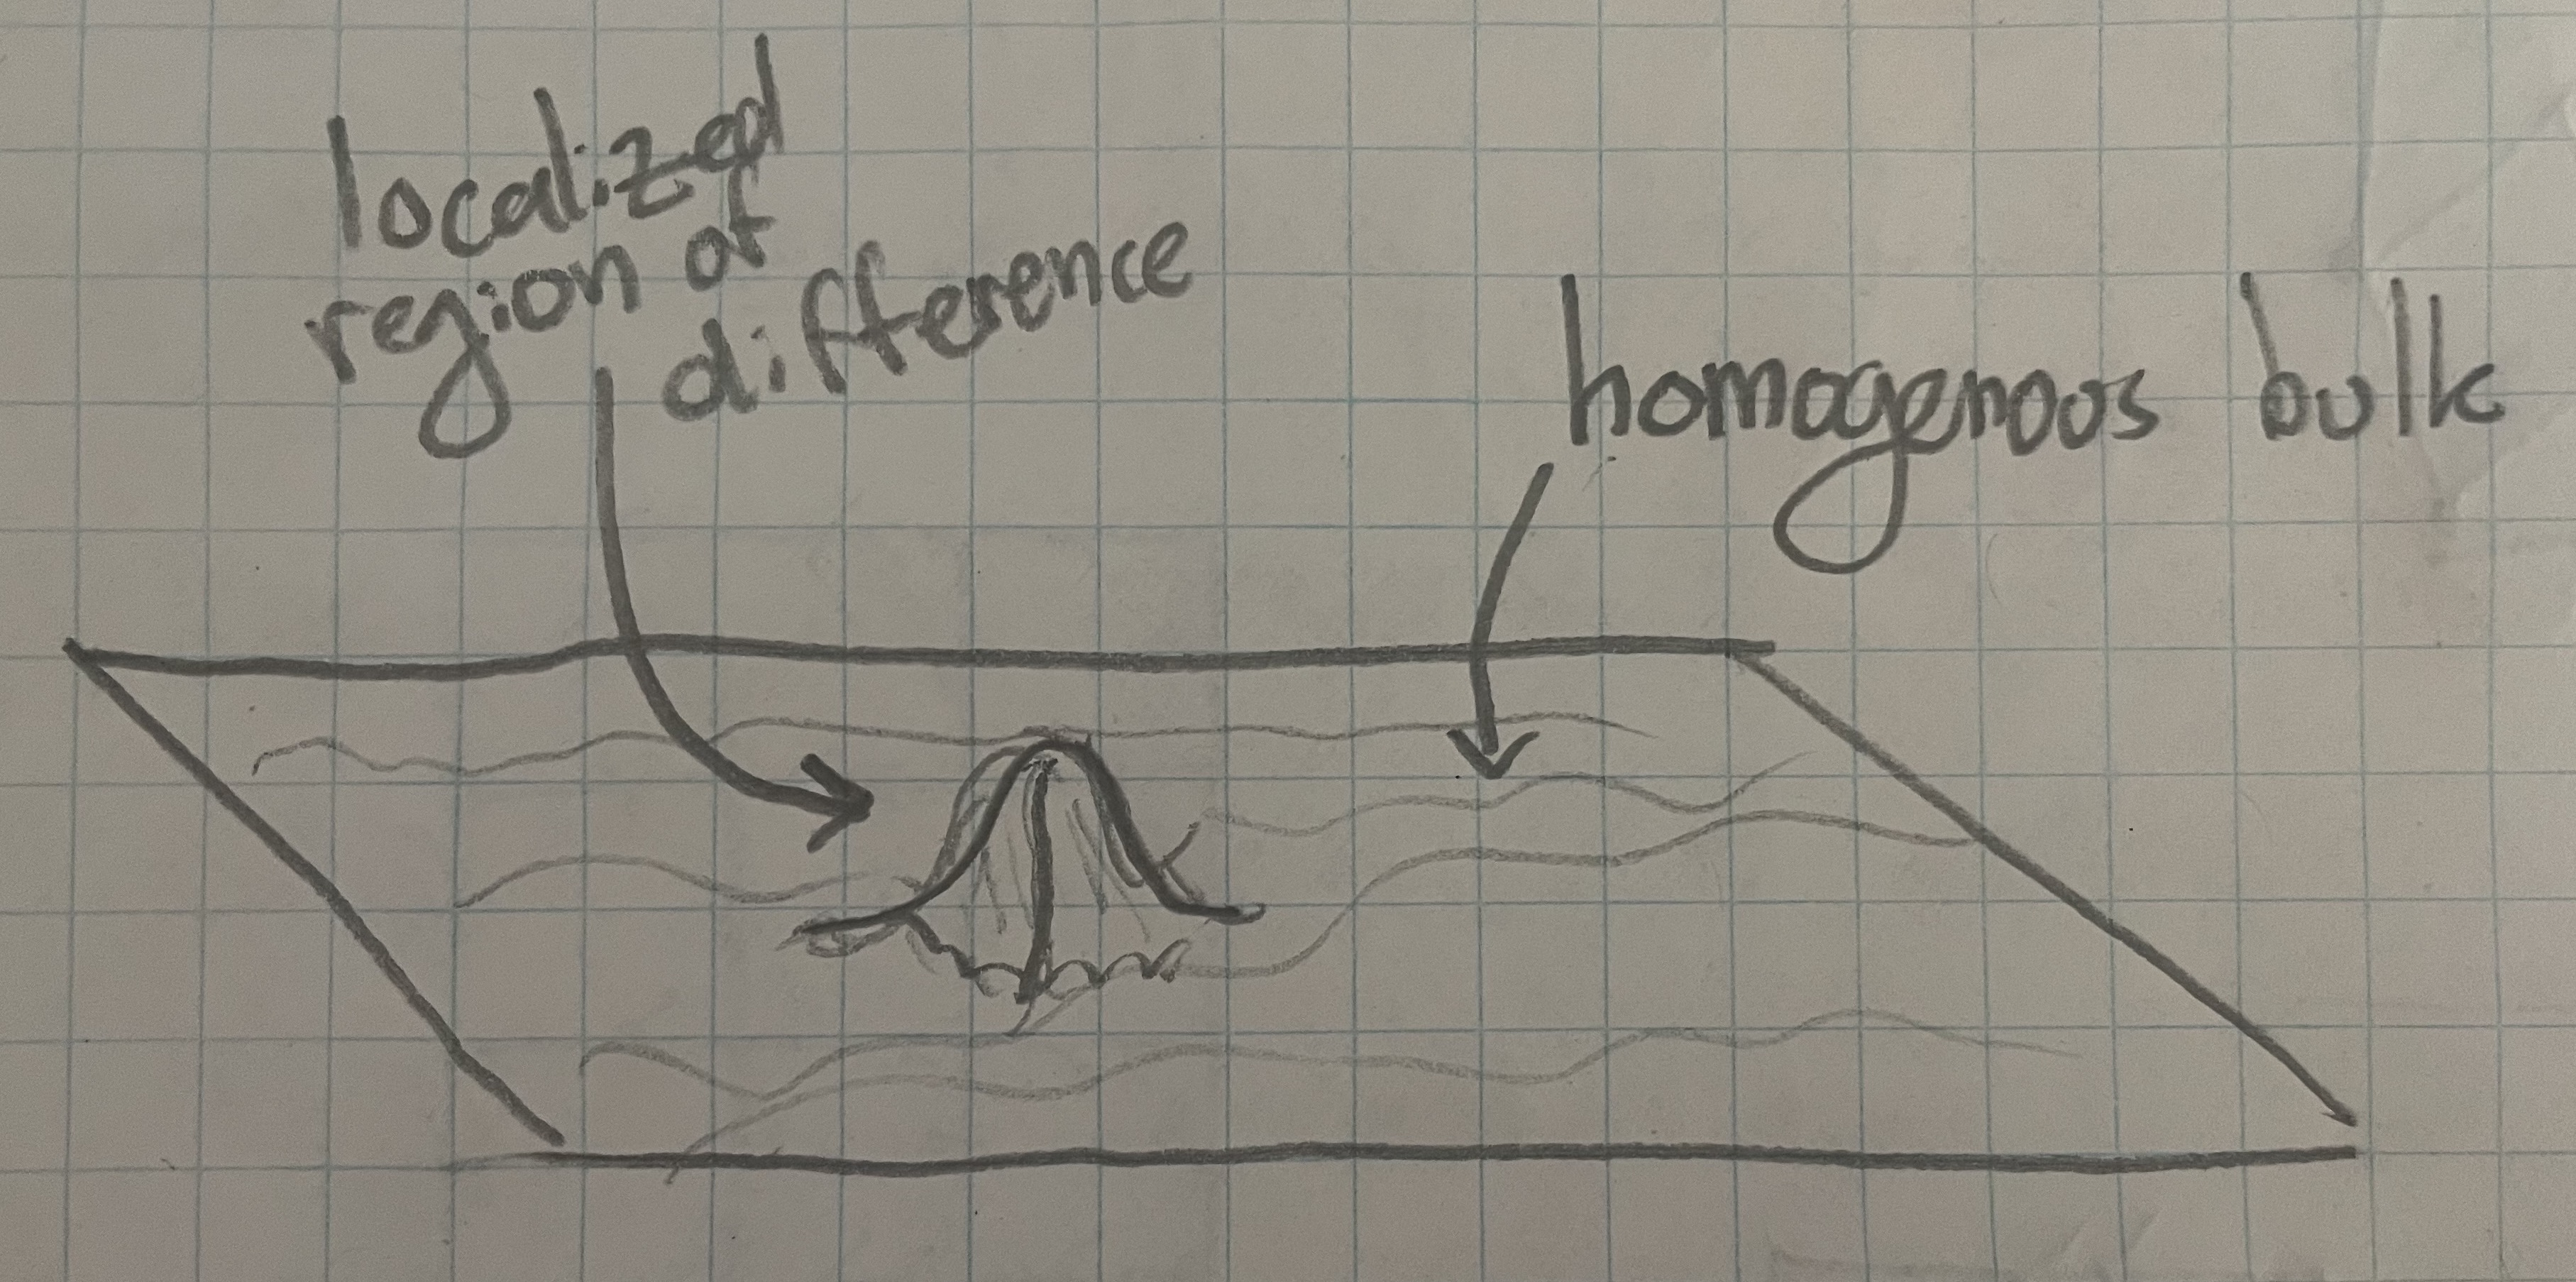
\includegraphics[scale=.04]{quasiparticle}
\end{center}
\caption{A quasiparticle in a two dimensional system}
\end{figure}

Our aim is to build a computer. In general this requires three components:

\begin{enumerate}
\item A method of storing information;
\item A method of manipulating information;
\item A method of reading out information.
\end{enumerate}

Information is stored in the state of the system - the bulk is described by some parameters, and the details of those parameters encodes information. Our method for manipulating information is \textit{braiding}. Braiding is the process whereby quasiparticles are moved along continuous paths around one another. There are two important points about braiding to keep in mind. The first is that braiding changes the state of the system. Even though the quasiparticles might be in identical places before and after the braid, the details of the system will change - there is more to the state of the system than just the positions of the quasiparticles. The second point is that the way that the state of the system changes depends \textit{only depends on the topology of the braid}, and not the geometry. Small deformations in the path taken by the quasiparticles do not affect the result - only global changes, like whether a path is taken clockwise or counterclockwise, makes a difference. This invariance is due to the fact that our system is topological. In geometric systems we expect the exact path taken by quasiparticles matters a great deal. The independence of the details of the paths is extremely specific to topological systems, and in the present setting is the \textit{defining topological feature}.

[WORK: add braid diagrams to demonstrate what braiding is like. Doesn't have to be string-diagram like - probably best to keep it in-plane 2D.]

At this point we can already see we have succeeded in our goal of making our computations fault-tolerant. Noise in the system will correspond to uncontrolled perturbations in the trajectories of the quasiparticles. This uncontrolled movement won’t change global properties of paths taken, and hence will not change the action of the braids on the system. That is, small errors won't affect computation! Of course, large enough errors could unintentionally make one quasiparticle wind around another. This would change the topology of the braid and hence ruin the computation. These errors are controllable, however, by moving the quasiparticles far apart and limiting the magnitude of the noise.

The final step in making our computer is to introduce a method for reading out information. This is done using \textit{fusion}. Fusion is the process whereby two quasiparticles are brought together, resulting in a single quasiparticle. In sufficiently complicated topological systems the result of fusion depends on the details of the state of the overall system. That is, the result of fusion can be used as a way of reading out information about the state! In its most basic form, when two quasiparticles fuse they can either result in a localized region which is identical to the homogenous bulk or is different from the homogenous bulk. If they result in a localized region identical to the bulk we say that the two quasiparticles have \textit{annihilated} each other. This can be seen as the difference between constructive and destructive interference. Two waves can either have destructive interference and annihilate each other when they meet, or they can have constructive inteference and result in a new wave. Measuring whether or not two quasiparticles annihilate upon fusion gives a method for reading out information.

In some situations, the result of fusion can even be nondeterministic. In this case the fusion can be repeated multiple times, which allows one to measure the \textit{probability} that two quasiparticles will annihilate each other. These probabilities are a rich source of data, and will serve as our way of reading out information in the current setting. The fact that our system is topological implies that the result of fusion does not depend on the specifics of the path taken, and hence this method of readout preserves the invariance of our computation to noise. This gives us a full picture of topological quantum computation, as seen in figure \ref{fig:TQC-outline}.

\begin{figure}
\begin{center}
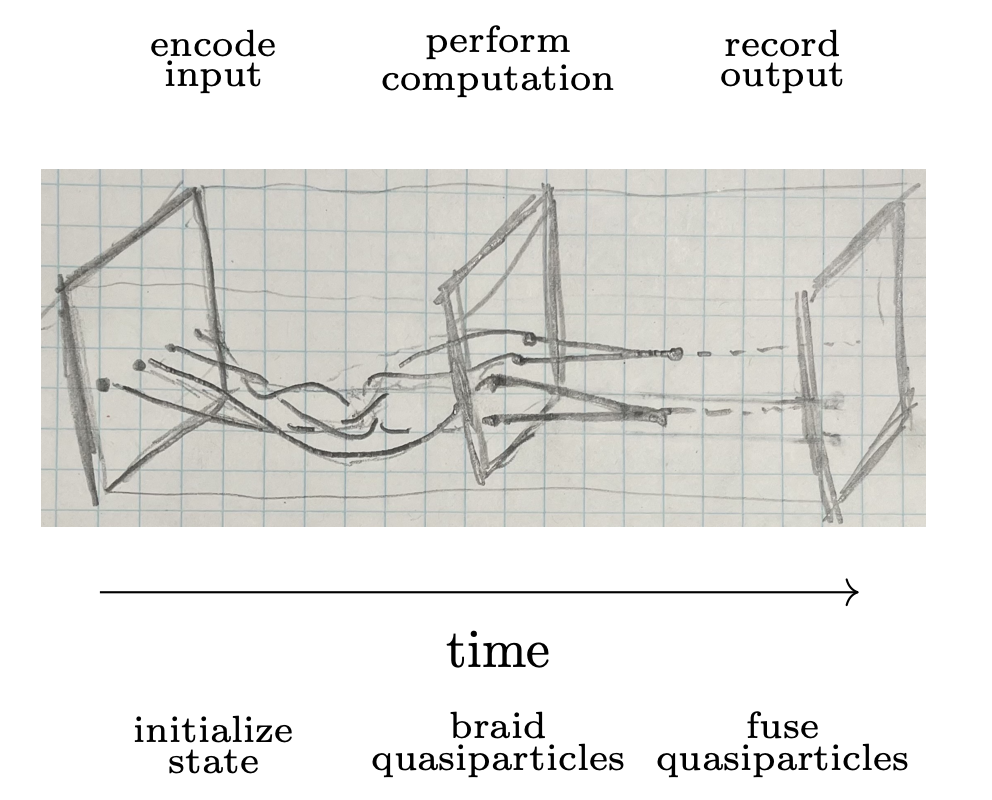
\includegraphics[scale=0.35]{TQC-outline}
\caption{A schematic of topological quantum computing}
\label{fig:TQC-outline}
\end{center}
\end{figure}

To make the above discussion more concrete, we will give a worked example. In this example we use a specific topological order known as the \textit{Fibonacci particle theory} to run Shor’s efficient quantum factorization algorithm \cite{shor1994algorithms}. The input of Shor’s algorithm is a positive integer. The output of Shor’s algorithm is the factorization of that integer. Shor’s algorithm is \textit{efficient} in the sense that it uses polynomially many quantum logic gates to arrive at its answer relative to the size of the input. Throughout this passage we will use \textit{efficient} and \textit{polynomially sized} interchangeably. The Fibonacci particle theory is a specific topological order, which describes in an algebraic fashion how the overall state changes when quasiparticles are braided and fused.

The first step in running Shor’s algorithm on a Fibonacci quantum computer is to translate the positive integer input into a certain braid. This is done using an efficient classical algorithm. The second step is to run this braid on a Fibonacci quantum computer. This is done by initializing some prescribed state and then braiding its quasiparticles. This initialization and braiding is performed repeatedly, and after every time two of the quasiparticles are fused. This lets us record a real number between 0 and 1, which is the probability that the two quasiparticles annihilate after the braiding. An efficient classical algorithm is then used to take this real number and obtain from it the factorization of the original input. Since all of these steps are efficient, it gives a topological quantum algorithm for factoring integers. The schematic for this process is shown below:

\begin{equation*}
\tikzfig{shor-fibonacci}
\end{equation*}

The magic in the above procedure is the existence of these two efficient classical algorithms: a first one for encoding integers into braids and a second one for decoding real numbers into factorizations. These algorithms are nontrivial. They are due to Freedman-Larsen-Kitaev-Wang \cite{freedman2002modular}. In fact, Freedman-Larsen-Kitaev-Wang showed that any problem which can be efficiently solved using a quantum circuit can also be solved using the Fibonacci particle theory, via a similar method of efficient classical preprocessing and postprocessing. It is in this sense that the Fibonacci theory is \textit{universal} for quantum computation.

The final step of this process would be to create a physical topological system which is described by the Fibonacci theory, which would serve as our quantum computer. In the realm of materials, the most promising approach seems to be to use specially tuned versions of the fractional quantum Hall system \cite{zhu2015fractional}. While these materials are theorized to host quasiparticles described by the Fibonacci theory, the difficulty of the experiment makes them inaccessible to current technology. There has been progress made on topological quantum error correcting codes which work by simulating the Fibonacci theory \cite{schotte2022quantum, schotte2022fault, xu2024non}. However these codes at the current moment have structural issues and require an unbearable amount of overhead to run, making them unfeasible to use on modern computers.

Progress on topological quantum computing has thus been focused on realizing topological particle theories other than the Fibonacci theory. These other theories can be constructed in more workable materials, and can be simulated as topological quantum error correcting codes with less overhead. The drawback of these other theories is that they are typically less computationally powerful, meaning that they require more tricks and techniques to achieve universal quantum computing. There are a great number of different proposals for how to achieve universal topological quantum computing, based on different particle theories, different methods of encoding information, different methods of manipulating information, and different methods of reading out information. It is an exciting time to be a theorist in the field of topological quantum information!

\subsubsection{Defects in ordered media}

We will now work through a complete mathematical example of a family of topological systems. Seeing as we don't assume that the reader is familiar with quantum mechanics, our examples will be \textit{classical} topological systems. Many of the important subtlties of topological quantum information are already present in the classical case. However, topological classical information is a smaller domain than topological quantum information - the reader should have a relatively complete grasp of the subject by the end of the chapter. Much of the discussion in this chapter is taken from an excellent review article by Mermin \cite{mermin1979topological}.

The family of systems we will describe goes by many names. In communities of experimentally focused physicists it goes by the name \textit{ordered media}. In mathematical physics communities it goes by the name \textit{classical field theory}. In pure mathematics it would be described as \textit{homotopy theory}. We will construct a system based on every topological space $M$. We will call $M$ the order space of our theory. We will assume throughout this chapter that $M$ is path connected.

To describe a system in physics, the first step is to define the space of possible states of the system. In this case, states will correspond to \textit{continuous maps $\phi: \RR^2\to M$}. We now give physical intuition for this choice of state space. The choice of $\RR^2$ as a source represents the underlying material. We are working on an infinite flat plane. Describing a function $\phi: \RR^2\to M$ amounts to choosing a value $\phi(x)$ for every point $x\in \RR^2$. In this way we imagine our system as being made up of infinitely many objects, one placed at each point in $\RR^2$, each of which has an internal state space $M$. Choosing the state of the overall system amounts to choosing the state of each individual object, that is, a value in $M$ for every point in the plane. The fact that $\phi$ must be continuous is a compatibility condition between the states of the objects at nearby points. It says that nearby objects must have similar states. We now list some examples which are described by this model:

\begin{itemize}
\item \textbf{Classical xy model of a 2D electron gas}. This model describes a possible behavior electrons in a flat 2D plane. An electron can be modeled as a point particle with a magnetic dipole pointing in some direction. This magnetic dipole is known as the \textit{spin} of the election, and can point in any direction in the plane. The topological space of all possible directions in the plane is a circle. Hence, in this system, the order space $M$ is the circle. The fact that nearby electrons must have similar spins is known as Hund’s rule, and is the most fundamental incarnation of ferromagnetism. It is physically derived as a consequence of the Pauli exclusion principle.

\item \textbf{Superfluid Helium-3} One famous example of ordered media is superfluid helium-3. Helium is an element. It has two stable isotopes: helium-3 and helium-4. The vast majority of helium on earth is helium-4, but there still is naturally occuring helium-3. At extremely cold temperatures helium-3 undergoes a phase transition, and becomes a superfluid. There are several different superfluid phases helium-3 can go into: B-phase, dipole-locked A-phase, dipole-free A-phase. For our purposes we will work with the dipole-locked A-phase. Its order space is $M=\SO(3)$, the group of rotations in three dimensional space.

\item \textbf{Biaxial nematics}. The objects at every point in the biaxial nematic should be thought of as small rectangles with unequal side lengths. These rectangles can be oriented in any direction in three dimensional space. In practice these objects will often be molecular compounds. They will not be exactly rectangular, but have the same symmetry group as a rectangle which is enough for the model to be accurate. To compute the space of possible orientations of a small rectangle, we work by the method of symmetries. Choosing some reference orientation to start with, every rotation in three dimensional space brings the rectangles to new orientations. The space of orientations of the rectangle is hence equal to $\SO(3)$ modulo the rotations which fix the rectangle. That is, $M$ is equal to $\SO(3)$ modulo the symmetry group of a rectangle.
\end{itemize}

[WORK: add diagrams for all three models]

We will now analyze these systems. In doing this analysis we will want to use the ideas of \textit{deformation} and \textit{topological equivalence}. Of course, these ideas are vague and require rigorous notions to make precise. We define these notions now. [WORK: this need to be reworded, with a proper caveat about rigor. Maybe bring up Jordan curve theorem for a laugh. Need to figure out what the policy on statements is.]

We now add a picture of \textit{dynamics} into our model - how it will be changing through time. In particular, we image that as time passes the system changes continuously. Let $\phi_t:\RR^2\to M$ be the state of the system at time $t$. We image that if $t_0$, $t_1$ are similar times then $\phi_{t_0}(x)$ and $\phi_{t_1}(x)$ will be close. Formally, this means that the maps $\RR_{\geq 0}to M$ assigning $t$ to $\phi_t(x)$ is continuous for all $x\in \RR^2$. This captures our intuitive notion of \textit{deformation}. We will image that the state of the system is constantly changing by deformations.

The first thing to notice about our system is that it is not storing any topologically-invariant information. In particular, every state can be continuously deformed to every other state. This is a general fact from topology: every pair of maps $\phi_0,\phi_1: \RR^2\to M$ can be continuously deformed from one to the other.

Clearly, this means that our system is not complicated enough to build a computer yet because it cannot store information. We rectify the situation by introducing quasiparticles. These quasiparticles go by many names. In the theory of ordered media they are known as defects. In field theory they are known as particles. In homotopy theory they are known as point singularities. For the sake of brevity, we will use the term defect.

A defect is a point at which we will drop our condition that the state $\phi:\RR^2\to M$ be continuous. This is done by making $\phi$ \textit{undefined} at certain points. Our new system is called \textit{ordered media with finitely many defects}. The state space consists of pairs $(S,\phi)$, where $S\subset \RR^2$ is a finite set and $\phi: \RR^2\\ S\to M$ is a continuous map.

[WORK: add picture of defects in ordered media]

Dynamics in our new system still correspond to continuous deformations. The subtelty now is that the defects can move as the state is deformed. We call these \textit{defect-mobile deformations}.

The vision for building our computer is that the experimenter should have control of the trajectories of the defects. This means that the system will trasform under defect-mobile deformations with definite paths chosen by the epxerimenter, but the details of the rest of the deformation is arbitarily and uncontrollable.

We can now outline the big idea of how the computer will work. We will arrange $n$ defects on a line in the plane. We keep these defects still, so that the system is changing only by deformations which keep the defects in place. We call these \textit{defect-fixed deformations}. We store our information in the possible configurations of this system:

[WORK: information storage space = (states with n defects arranged in a line)/ (defect-fixed deformation)]

The way we act on this information is by moving the defects around each other. This movement of defects induces some defect-mobile deformation. The space we are storing our information in is invariant under defect-fixed deformation, but not defect-mobile deformations. Hence, moving the defects around non-trivial paths will have non-trivial action on the stored information. This action on stored information is exaclty how we perform our computations.

Finally, we must introduce a method for reading out information. This is done via fusion. Two defects can be brought together and fused. The result of this fusion is a topologically invariant quantity, and we will assume that it can be measured by an experimenter. In its most simple form, this amounts to detecting whether two defects annhilated or not.  This gives us some information about the state, which is the output of our computation.

[WORK: add schematic for this process]

In the rest of this chapter we will describe exactly what the space we are storing our information in looks like, how braids act on that information, and how this can be used to make a functioning computer. This will give a detailed picture of how topological computation works.

\subsubsection{The fundamental group}

To understand topological computation in ordered media we will need to put in some real work in analysing the system, and make some non-trivial observations. The structure of this analysis will be largely the same as the analysis which will be taking place throughout the rest of this book. We recall the overall outline of this text, which goes as follows:

[WORK: add outline.]

In this section we will do a very similar thing. We will take our physical model, ordered media, and take its algebraic description. That algebraic description can then be used for making a computer. Luckily for us, the algebraic theory underlying ordered media is much simpler than the algebraic theory underlying topological order: it's group theory. In particular, we will even assume that all relevant groups are \textit{finite}. In this way, modular tensor categories can be seen as vast quantum generalizations of finite groups. The schematic in our case is shown below:

[WORK: add outline w/ group theory instead of MTC.]

The way we go from defects in ordered media to group theory is by using a construction known as the \textit{fundamental group} from homotopy theory.

The fundamental group is derived from a careful analysis of loops in topological spaces. We first clairfy what we mean by \textit{loop}. Loops, for our purposes, are always \textit{oriented} and are allowed arbitrary self intersections. Examples of loops around a point are shown below:

[WORK: add pictures of loops.]

Formally, we define a loop in a topological space $M$ to be a continuous map $\alpha:[0,1]\to M$ such that $\phi(0)=\phi(1)$. Our main goal us to understand topological information. Topological information is stored in properties which are invariant under deformations. Hence, we are naturally interested in the space of loops up to deformation.

In the plane $\RR^2$ with a point removed, points up to deformation are classified by their \textit{winding number}. This winding number is an integer which says how many times the loop went around the point. This windingn number is an integer in $\ZZ$, with positive numbers corresponding to counterclockwise rotations and negative numbers corresponding to clockwise rotations. The loops in figure [ref] have their winding numbers given as an illustration of the concept.

The key ingredient we are missing is the \textit{group structure}. We want to get groups out of topological spaces, but so far all we have is a set. The group structure comes from composition. Given two loops we can compose them by first following one loop and then following the othe. In this language, we see the topologists' winding-number version of $1+1=2$ below:

[WORK: add 1+1=2 with winding numbers.]

This definition has a big problem though. To compose, we need to choice a point to start and stop two two loops being composed at. This special starting/stopping point is known as a \textit{basepoint}. This deal of choosing basepoints is very important for the theory. Formally, a loop in $M$ based at $m\in M$ is a map $\alpha:[0,1]\to M$ such that $\phi(0)=\phi(1)=m$. We define the composition of two loops $\alpha_0,\alpha_1$ in $M$ based at $m\in M$ to be

$$
(\alpha_1 \circ \alpha_0)(t)=
\begin{cases}
\alpha_0(2t) & 0\leq t \leq 1/2 \\
\alpha_1(2(t-1/2)) & 1/2 < t \leq 1.
\end{cases}$$

The reason we need to add the factors of $2$ is to ensure that the domain of the loop is still the unit interval $[0,1]$. Intuitively, to fit two loops in the same amount of time we had to speed-up both loops by a factor of 2.

We are now almost ready to define the fundamental group: we have defined based loops, and we have defined a rule for their composition. The last subtelty is in discussing what it means to deform based loops. In particular, should deformations be allowed to move the basepoint? The issue that we want to be able to compose our loops. To compose loops they need to have the same basepoint. If the basepoint moves then we will lose out composition structure. Hence, for the time being, we should only work with deformations which preserve the basepoint. With this subtelty out of the way, we can finally define the fundamental group. Given any connected topological space $M$ and any point $m\in M$, we define the \textit{fundamental group of $M$ based at $m$} to be the group

$$\pi_1(M,m)\coloneqq \left(\text{loops in $M$ based at $m$}\right)/\left(\text{basepoint preserving deformations}\right)$$

whose group structure is given by the composition of based loops. As an example, our earlier comments about loops around points can be summarized as the statement that $\pi_1(\RR^2\backslash\{p\},b)\cong \ZZ$ for any distinct points $b,p\in \RR^2$. The identity element in the fundamental group is the trivial loop which stays at its basepoint and doesn't move (formally, the constant map $\alpha:[0,1]\to M$), and inverses are given by reversing orientation (formally, the inverse of $\alpha:[0,1]\to M$ is $\alpha^{-1}(t)=\alpha(1-t)$.)

We can now start to use the fundamental group to analyse defects in ordered media. The first major insight is that loops in physical space yield loops in order space. Let $S$ be a finite set of defects and let $\phi: \RR^2 \backslash S \to M$ be a state. Given any loop $\alpha$ in $\RR^2\backslash S$ based at $b\not\in S$, postcomposing with $\phi$ gives a loop in $M$:

$$(\phi \circ \alpha): [0,1]\xrightarrow{\alpha} \RR^2 \backslash S \xrightarrow{\phi} M.$$

This loop has basepoint $(\phi \circ \alpha)(0)=(\phi\circ \alpha)(1)=\phi(b)$. This gives an element of $\pi_1(M,\phi(b))$. Given any state $\phi$ and given any loop $\alpha$ based at $b$, we call the corresponding element of $\pi_1(M,\phi(b))$ the \textit{winding number of $\phi$ along $\alpha$}. This sort of winding number generalizes the standard notion of a winding number of a loop around a point discussed before.

Now, consider the system with $n$ defects arranged in a line. We can choose a basepoint $b$ above all of the defects. We add loops $\alpha_i$ based at $b$ for each $1\leq i \leq n$, each of which go directly around defect $i$ counterclockwise exactly once. This is depicted visually below:

[WORK: add picture.]

Given any ordered state $\phi$ on this system, we can take the winding numbers of each loop $\{\alpha_i\}_{i=1}^n$. These winding numbers all live in $\pi_1(M,\phi(b))$. Hence, to each state we can assign an element in the $n$-fold Cartesian product $\pi_1(M,\phi(b))^n$.

Fantastically, the values in $\pi_1(M,\phi(b))^n$ change in a well-behaved way under braids. We use a $2$-defect system to illustrate the principle.

[WORK: add good pictures to show why making $g_1$ go under $g_2$ maps $(g_1,g_2)$ to $(g_2,g_1)$. Talk a bit about it in words too]

This gives us a picture for how our computer works: information is stored in the winding numbers of the defects, and braiding acts by conjugating the winding numbers by each other.

There are a still a few lingering points that need to be sorted out before we can start building our computer. The first is the issue of whether our information being stored is actually invariant under defect-fixed deformations. Unfortunately, it is \textit{not}. The problem is that deformations in general have no reason to preserve the value of $\phi(b)$. The deformations will hence change the basepoints. However, elements of the fundamental group are only defined up to basepoint-preserving deformations! Hence, deformations of the state will change its winding numbers. In general we have the following key relation:

$$\left(\text{loops in $M$ based at $m$}\right)/\left(\text{basepoint preserving deformations}\right)= \pi_1(M,m)$$

$$\left(\text{loops in $M$ based at $m$}\right)/\left(\text{arbitrary deformations}\right)= \left(\text{conjugacy classes in }\pi_1(M,m)\right).$$

The intution for this above fact is as follows. Let $\alpha$ be a loop based at $b$. Let $\alpha'$ be the same loop but with a different choice of basepoint $b'$. Let $\epsilon$ be the portion of the loop between $b$ and $b'$. Going along $\alpha$ is the same as first going along $\epsilon$ to get to $b'$, then going along $\alpha'$, and then going along $\epsilon^{-1}$ to get back to $b$. Hence, we have $\alpha = \epsilon^{-1}\circ \alpha' \circ \epsilon$. Hence, choosing different basepoints amounts to conjugation. This is illustrated below:

[WORK: add diagram]

All this is to say that the winding numebrs in an $n$-defect ordered media state $\phi$ are not preserved up to defect-fixed deformations. Properly dealing deformations requires properly keeping track of conjugacy classes versus group elements. This sort of effort, however, is unnececary because it does not change any of the key takeways or any of the important concepts. Hence, \textit{we will assume that all of our deformations do not change the value of $\phi(b)$}. We will choose some element $m\in M$ and assume $\phi(b)=m$ is fixed. For physical motivation, one can imagine moving the basepoint far away towards infinity. Since all of our physics is local we can imagine that the magnitute of the deformations go to zero away from the origin and hence the point at infinity is preserved by all local nosie.

Our last subtelty to discuss is reading out information. As we have just discussed, the values of the winding numbers in $\pi_1(M,m)$ are very dependent on the choice of basepoint. This means that the information encoded in this winding number is spread out over the whole region between the defect and the basepoint. This nonlocal nature makes it hard to measure, especially when the basepoint is taken away towards infinity. The readily measurable local information is the non basepoint-preserving winding number of the loop around defects. That is, the conjugacy classes in $\pi_1(M,m)$ associated to the defects. These conjugacy classes should be measurable in a reasonable experimental setup.

However, as we braid, these conjugacy classes do not change, and hence the outcomes of our measurments won't be affected. In a way, this is the point - braiding can change the spread-out global topological information, but will not change local quantities, like the conjugacy class in $\pi_1(M,m)$. In this way we can think of the conjugacy class as a well-defined \textit{type} of the defect, whereas the exact value in $\pi_1(M,m)$ is a global quantity which depends on the choice of basepoint

The way to get around this issue is to fuse the defects before braiding. Fusing defects together amounts to bringing them close together until they act like a single defect. If the defects have winding number $g_1,g_2$, then their fused defect will have winding number $g_1g_2$ as illustrated by the below diagram:

[WORK: add diagram.]

Hence, given a state $(g_1,g_2... g_n)$, the measurable quantities are the conjugacy classes of products of adjacent defects. For instance, fusing all of the defects one-by-one to the left would allow one to measure the conjugacy classes of $g_1$, $g_1g_2$, $g_1g_2g_3$, all the way up to $g_1g_2g_3...g_n$.

This completes our analysis of defects in ordered media based on the fundamental group.

\subsubsection{Topological classical computation}

We are now ready to describe the theory of topological classical computation. In the previous section, we showed how all of the topological information of defects in ordered media is controlled by the fundamental group $G=\pi_1(M,m)$ of the order space $M$ relative to some basepoint $m\in M$. This is the heart of the algebraic theory of topological computing. Even though our physical model is complicated, the algebraic data can be succicntly summarized as a single group $G=\pi_1(M,m)$. In this way, we will formulate our discussion of topological classical computation in a way which does not make reference to the order space at all. We will choose an abstract group $G$ and make a computer using it.

On a purely mathematical level we don't need to make any restrictions on the group $G$. It is a theorem from homotopy theory that every group is the fundamental group of some topological space. However, we will make restrictions on our choice of group coming from physical concerns. We will ask that our group be \textit{finite}. A first reason for this is error protection. Suppose that $G$ were some continuous group, like $G=\RR$. If the stored information was $\pi=3.1415...$, it would be difficult for this information to not drift to $3.1416...$. Even though there aren't any continuous deformations which would change a winding number, small non-continuous deformations could still make this sort of jump. For this reason it is preferable to work with \textit{discrete} groups - groups whose natural topology is discrete. Discreteness implies a degree of seperation, which means that winding numbers will not spontaneously jump from one element to the next. This gives the system error resistance.

The choice to make the group finite is more subtle. For instance, $G=\ZZ$ appears in many physically reasonable contexts. Our choice mainly steps from the practical consideration that finite groups are simpler to work with than infinite ones, and the general physical principle that symmetry groups should be compact. Any compact discrete group must be finite. This compactness argument will become especially relevant once we pass to quantum mechanics.

In summary, the algebraic theory of topological classical information we present is really just a special case of finite group theory, which is a well understood subject.

Our systems will consist of $n$ defects on a straight line. These defects will be labeled with group elements $g_i\in G$, for $1\leq i \leq n$. We recall that these labels correspond to winding numbers around loops:

[WORK: add diagram.]

Braiding $g_i$ under $g_{i+1}$ amounts to replacing $g_i$ with $g_{i+1}$, and replacing $g_{i+1}$ with $g_{i+1}^{-1}g_i g_{i+1}$. Fusing the defects $g_{i}$ and $g_{i+1}$ amounts to replacing them with a single defect labeled $g_{i}g_{i+1}$. The \textit{type} of a defect is the conjugacy class of its label in $G$. These types are local observables which can be measured by the experimenter.


[WORK: add little pictures summarizing these rules]

This leads to the very natural question: \textit{for which groups $G$ can I make a full classical computer?} This is a design problem in finite group theory.

Our first step towards answering it is making a closer analysis of how braiding works. We define the braid group as our main tool:

[WORK: Bn = ways of braiding n points around each other/endpoint-preserving deformations. Define Pn too. Also give examples. Maybe this is where to introduce the graphical language, things going thru time?]

Every braid can be made up piece-by-piece using indivudal swaps. Let $\sigma_{i}$ denote the swap which sends the point at positoin $i$ under the point at position $i+1$. The group $B_n$ is generated by the $\sigma_i$, for $1\leq i \leq n-1$. We observe that the following two braids can be deformed from one to the other:

[WORK: add Yang-Baxter braid]

Algebraically, this is the identity $\sigma_{i}\sigma_{i+1}\sigma_{i}=\sigma_{i+1}\sigma_{i}\sigma_{i+1}$. Additionally, if $i$ and $j$ are not adjacent, that is $|i-j|\geq 2$, then $\sigma_{i}\sigma{j}=\sigma_j\sigma_i$ as seen in the below picture:

[WORK: far-commutivity picture.]

This yields the algebraic fact that

$$B_n=\left<\left.\sigma_1,\sigma_2,...\sigma_{n-1}\right| \substack{\sigma_{i}\sigma_{i+1}\sigma_{i}=\sigma_{i+1}\sigma_{i}\sigma_{i+1}, \\ \sigma_i\sigma_j=\sigma_j\sigma_i}\,\,\,\,\forall 1\leq i,j \leq n-1,\,\, |i-j|\geq 2\right>.$$

It is at this point that we can move past our non-rigorous topological considerations for braiding. The lack of rigor in our treatment of braid groups and our lack of rigor in our treatment of defect trajectories cancel, giving us our first well-formed mathematical proposition. It encodes the fact that moving defects by braids acts on the stored information:

\begin{proposition} Let $G$ be a finite group, and let $n\geq 1$ be an integer. The map

\begin{align*}
\rho_n: B_n &\xrightarrow{} \Sym\left(G^n\right)\\
\sigma_i &\mapsto \left((g_1... g_i, g_{i+1} ... g_n)\mapsto (g_1... g_{i+1}, g_{i+1}^{-1}g_i g_{i+1} ... g_n) \right)
\end{align*}

defines a homomorphism of groups between the braid group $B_n$ and the group of set-wise permutations of the Cartesian product $G^n$, $\Sym(G^n)$.
\end{proposition}
\begin{proof}.[WORK: do proof]
\end{proof}

The dream would be that braids alone would be enough for universal classical computation. For instance, suppose that $G$ is a finite group with a conjugacy class $C$ that has order $2$. Identifying $C\cong \{0,1\}$ as a set, we can identity $C^n\cong \{0,1\}^{n}$ with $n$-bit strings. Suppose the homomorphism $\rho_n:B_n\to \Sym\left(C^n\right)\cong \Sym(\{0,1\}^n)$ were surjective. This would mean that every element of $\Sym(\{0,1\}^n)$ could be written in terms of braids on $G$. In the language of computer science, maps $\{0,1\}^n\to \{0,1\}^n$ are called \textit{boolean functions}. The surjectivity of the braid group homomorphism would say that every bijective boolean function could be implemented by braiding defects, and hence every bijective computation could be done using braiding. Bijective boolean functions in the world of computation are known as \textit{reversible}. Most problems we care about are not inversible. For instance, adding integers is not reversible because multiple summands could give the same sum as demonstrated in $1 + 3 = 2 + 2 = 4$.

This leads to two problems to deal with:

\begin{enumerate}
\item Braids can only ever give reversible computations. This is not a major issue because it's known that there is an efficient clever way of turning every non-reversible computation problem into a reversible one \cite{bennett1973logical}. However, reversibility is still cumbersome and annoying.

\item There aren't any groups $G$ which have conjugacy classes $C$ for which the map $\rho_n: B_n \to \Sym\left(C^n\right)$ is surjective.This is because, for instance, choosing some $x\in C^n$ we could have the whole input be a string of all $x$: $(x)_{i=1}^n\in C^n$. Since $x$ commutes by itself and the braid group acts by conjugation, every braid will act trivially on this input. Hence, $\rho_n(\beta)\left((x)_{i=1}^n\right)=(x)_{i=1}^n$ for every braid $\beta\in B_n$. There is no way to make a nontrivial computation from braiding if all inputs commute. 

\end{enumerate}

The way around the problem of commuting inputs is to use pair-creation. Just like how at any time two defects $(g_1,g_2)$ to make the defect $g_1g_2$, at any time this process could reverse and out of nothing the pair of defects $(g,g^{-1})$ could be created. The important part of this process is that $g$ can be chosen so that it does not commute with the inputs.

[WORK: add a bit of explanation about this, introducing all the ingredients we need]

We now have all of our ingredients, we can finally state our main results about making computers. Clearly, if $G$ is abelian then it won't be useful for making a computer. Our computer is based on acting by conjugation, and conjugaction is trivial in abelian groups. However, just being nonabelian is not enough. The group needs to be \textit{sufficiently non-abelian} so that conjugation is powerful enough to implement any computation possible.

We define the subgroup

$$[G,G]=\{\text{subgroup of $G$ generated by elements of the form }g_{0}g_{1}g_{0}^{-1}g_{1}^{-1}\text{ for }g_0,g_1\in G\}.$$

The subgroup $[G,G]$ is called the \textit{commutator subgroup} of $G$, and the elements $g_{0}g_{1}g_{0}^{-1}g_{1}^{-1}$ are called commutators. Clearly, if $G$ is abelian then all of its commutators are trivial and hence $[G,G]=0$. To make a good computer, we need sufficiently many commutators. In fact, we need the following condition: $[G,G]=G$. For technical reasons it also easiest to assume that $G$ is \textit{simple}. That is, it has no proper nontrivial normal subgroups.

We observe that every non-abelian simple group is automatically perfect. This follows from the fact that the commutator subgroup $[G,G]$ is a normal subgroup of $G$. Since $G$ is nonabelian the commutator subgroup $[G,G]$ is nontrivial, and since the only nontrivial subgroup of $G$ is itself we get that $[G,G]=G$.

In this case we have the following important result:

\begin{theorem}[Mochon] . [WORK: I want a good statement of Mochon's theorem, need to think more about it and read Mochon's paper again. State it as ``for every non-abelian simple group $G$".]
\end{theorem}
\begin{proof} . [WORK: do proof.]
\end{proof}

We can now give a full example of how this works. [WORK: give a full example, using $G=A_5$. Of course, full is a tricky word here. Enough to make what's going on clear to people.]

Now that we know how to make a universal computer, we can analyse how the power of computation changes as $G$ is chosen to be more or less abelian. The general theme is that if a group is more non-abelian then it will have more computaional power. Of course, being ``more" or ``less" abelian is not a well-defined term. We introduce here some formal notions from group theory which measure abelianness.

If a group is very nonabelian it should have a big commutator subgroup. That is, $[G,G]$ should be large in a certain sense. One way for this to be true is for the group to be perfect, that is, $[G,G]=G$. A weaker condition is that $G$ should have a perfect subgroup - a subgroup $H\leq G$ such that $[H,H]=H$. Intuitively, it makes sense that any group with a perfect subgroup should be useable for universal topological computatoin. You can just focus on the perfect subgroup and use Mochon's theorem, and forget about the rest of the group. A group with a perfect subgroup is called \textit{non-solvable}.

There is another useful step to consider between non-solvable and abelian. Some groups $G$ have subgroups $H$ such that $[H,H]$ might be small, but $[H,G]$ is bigger. When $H$ is allowed to take commutators with elements of $G$ you get potentially more elements, so $[H,H]\leq [H,G]$. When $H$ is a normal subgroup, we find that $[H,G]\leq H$ since for all $h\in H$, $g\in G$, the commutator

$$g h g^{-1} h^{-1}= (g h g^{-1}) h \in H$$

since $(g h g^{-1}) \in H$ by the normality of $H$ and $h\in H$ by assumption. If $G$ has a normal subgroup $H$ such that $[H,G]=H$, we call $G$ \textit{non-nilpotent}. Clearly we have the following inclusioins:

$$
\left(\substack{\text{non-solvable} \\ \text{groups}}\right)\subset
\left(\substack{\text{non-nilpotent} \\ \text{groups}}\right)\subset
\left(\substack{\text{non-abelian} \\ \text{groups}}\right).
$$

This induces a hierarchy of adjectives, from most abelian to least abelian:

\begin{equation*}
\tikzfig{hierarchy-of-adjectives}
\end{equation*}


The following phenominon presents itself. We find that less abelian a group is the more computational power it has. Additionally, the more computational power it has the harder it is to create topological systems in the lab which are algebraically described that group. It is harder to make systems which make good computers.

This phenominon is especially well developped in the quantum case. Given a finite group $G$, we can describe a classical system of ordered media based on $G$. This system can be \textit{quantized}. This turns it into a topological quantum system whose behavior is still goverened by the group $G$. This quantized system is known as the \textit{quantum double} of $G$, and is denote $\D(G)$. These systems behave very similarly to the ones discussed in this chapter, just made quantum. These quantum doubles and the algebraic theory describing them and their generalizations will be the topic of much of this book.

In the case of quantum doubles we can make a table detailing exactly the relationship between level of abelianness, computational power, and experimental status:

[WORK: need to introduce universality as a concept]

\begin{center}
\begin{tabular}{|| c | c | c | c ||} 

\hline
Abelianness & Smallest Example& Computational power of $\D(G)$& Experimental Status \\ [0.5ex] 
 \hline\hline
  &  & &\\ 
 non-solvable & $G=A_5,$ & Straightforwardly universal.& Fundamental limitations\\
  & alternating group & (Chapter [ref], \cite{mochon2003anyons})& coming from intensive\\ 
  & with $|A_5|=60$ & & circuit-depth requirements,\\ 
  &  & & and the size of the.\\ 
  &  & & smallest example.\\ 
  &  & & (\cite{bravyi2022adaptive}).\\ 
  &  & &\\ 
 \hline
  &  & &\\ 
 solvable& $G=S_3,$ & Universal with tricks. & Has yet to be done.\\
 non-nilpotent& symmetric group& (Chapter [ref], \cite{mochon2004anyon}) & There are some inherent \\ 
 & with $|S_3|=6$ & & difficulties involved.\\ 
  &  & & (\cite{tantivasadakarn2023hierarchy})\\ 
  &  & &\\ 
 \hline  &  & &\\ 
 nilpotent& $G=D_4,$ & ? & Preliminary experiments \\
 non-abelian& dihedral group & & have been successful.  \\ 
 & with $|D_4|=8$ & & (\cite{iqbal2024non})   \\ 
  &  & &\\ 
 \hline
  &  & &\\ 
 abelian & $G=\ZZ_2,$ & Universal schemes seem& Widely used\\ 
  & cyclic group & to be impossible.& in most applications. \\ 
  &with $|\ZZ_2|=2$ &  Non-topological methods& (\cite{bravyi2024high, hong2024entangling}\\ 
  &  & seem to be required.& \cite{balewski2024engineering, google2023suppressing})\\ 
  &  & (Chapter [ref], \cite{bravyi2013classification, eastin2009restrictions}) &\\ 
  &  & &\\ 
 \hline
\end{tabular}
\end{center}

We make a few comments about this table.

\begin{enumerate}
\item We notice that difficulty inherent to experimentally realizing topological phases is \textit{not} completely controlled by the size of that group. The quantum double $\D(D_4$) is simpler to realize than $\D(S_3)$ because it is nilpotent and $S_3$ is not, despite the fact that $|D_4|=8$ is larger than $|S_3|=6$.

\item All of the experimental results cited come from the side of topological quantum error correction and not topological quantum materials. This is because most topological quantum materials are described by algebraic theories which are not doubles of finite groups. Doubles of finite groups are primarily used in topological quantum error correction theory.

\item This table details a general programme. Given an algebraic theory of topological information, there is the question of how to make a universal quantum computer. The culmination of this book is Chapter [ref], where we show describe six different families of algebraic theories and show how to make a universal quantum computer out of all of them.

\end{enumerate}

This concludes our overview of the subject!

$\newline\newline$

\large \textbf{Exercises}:\normalsize

\begin{enumerate}[\thesection .1.]

\item .[WORK: show that simulability $\implies$ \textit{efficient} simulability. Do the work in the case $G=A_5$]

\item .[WORK: show that nilpotent $\implies$ polynomial growth? Can reference the more general picture of size of braid group images.]

\end{enumerate}


